%----------------------------------------------------------------------------
\appendix
%----------------------------------------------------------------------------
\chapter*{F�ggel�k}\addcontentsline{toc}{chapter}{F�ggel�k}
\setcounter{chapter}{6}  % a fofejezet-szamlalo az angol ABC 6. betuje (F) lesz
\setcounter{equation}{0} % a fofejezet-szamlalo az angol ABC 6. betuje (F) lesz
\numberwithin{equation}{section}
\numberwithin{figure}{section}
\numberwithin{lstlisting}{section}
%\numberwithin{tabular}{section}

\begin{figure}[!ht]
	\centering
	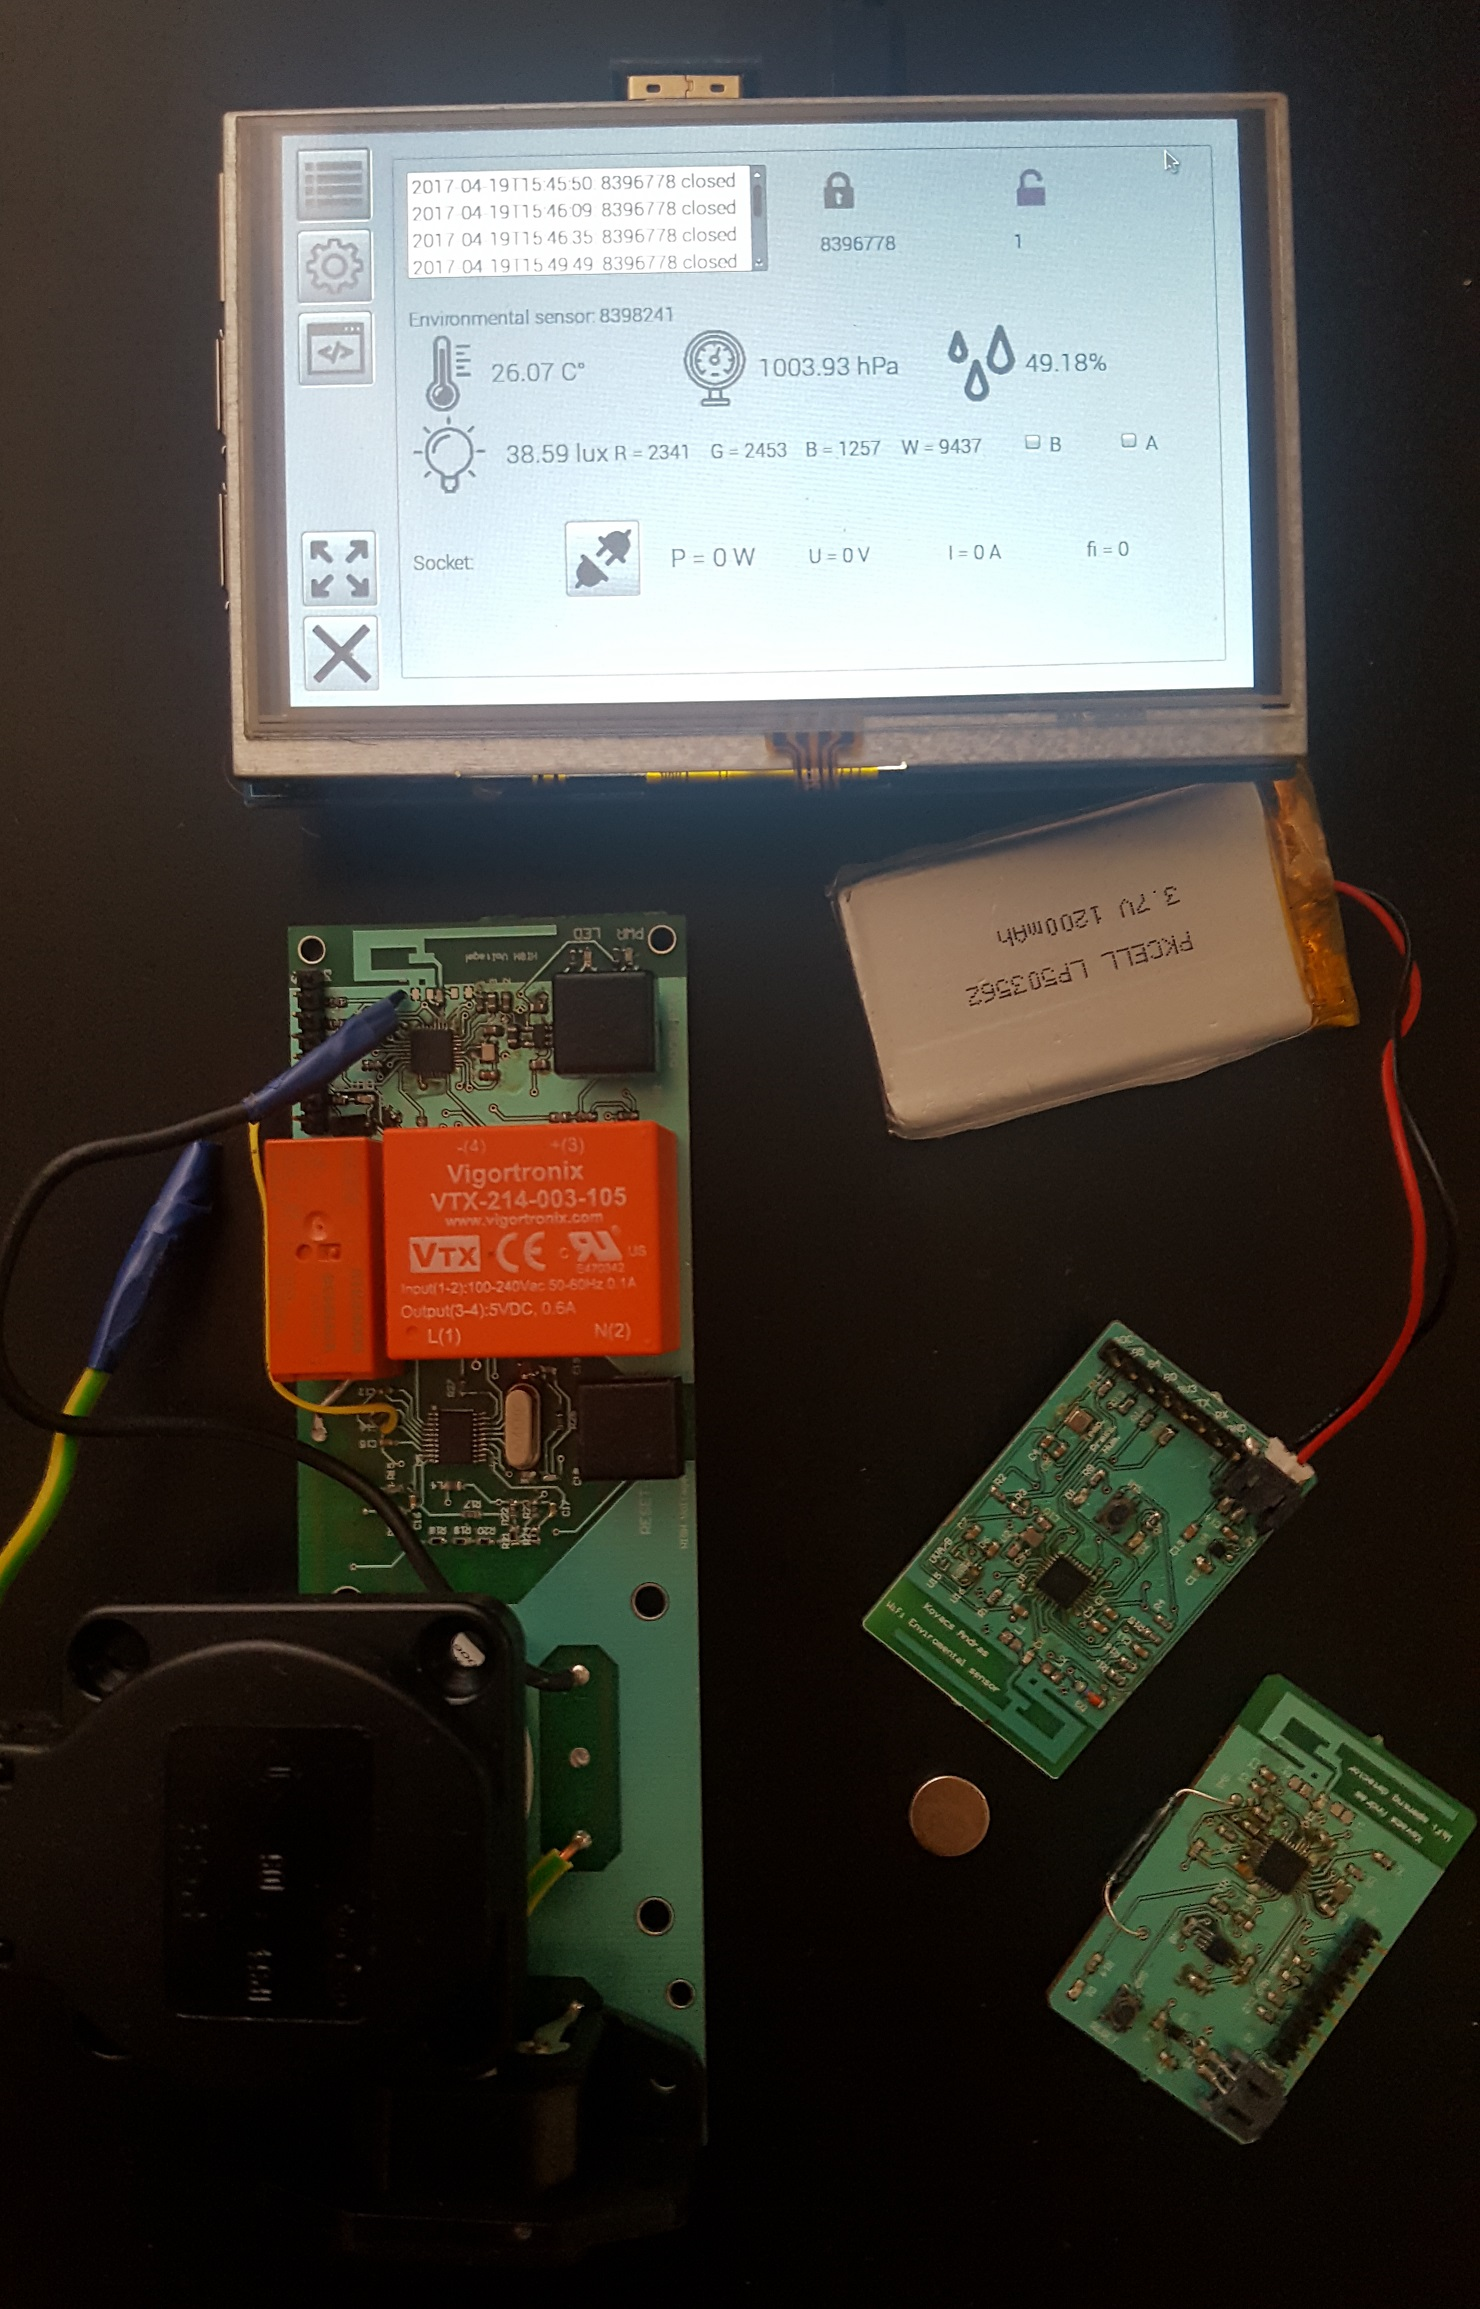
\includegraphics[width=150mm, keepaspectratio]{figures/device-all.jpg}
	\caption{Az elk�sz�lt rendeszer} 
\end{figure}

\begin{figure}[!ht]
	\centering
	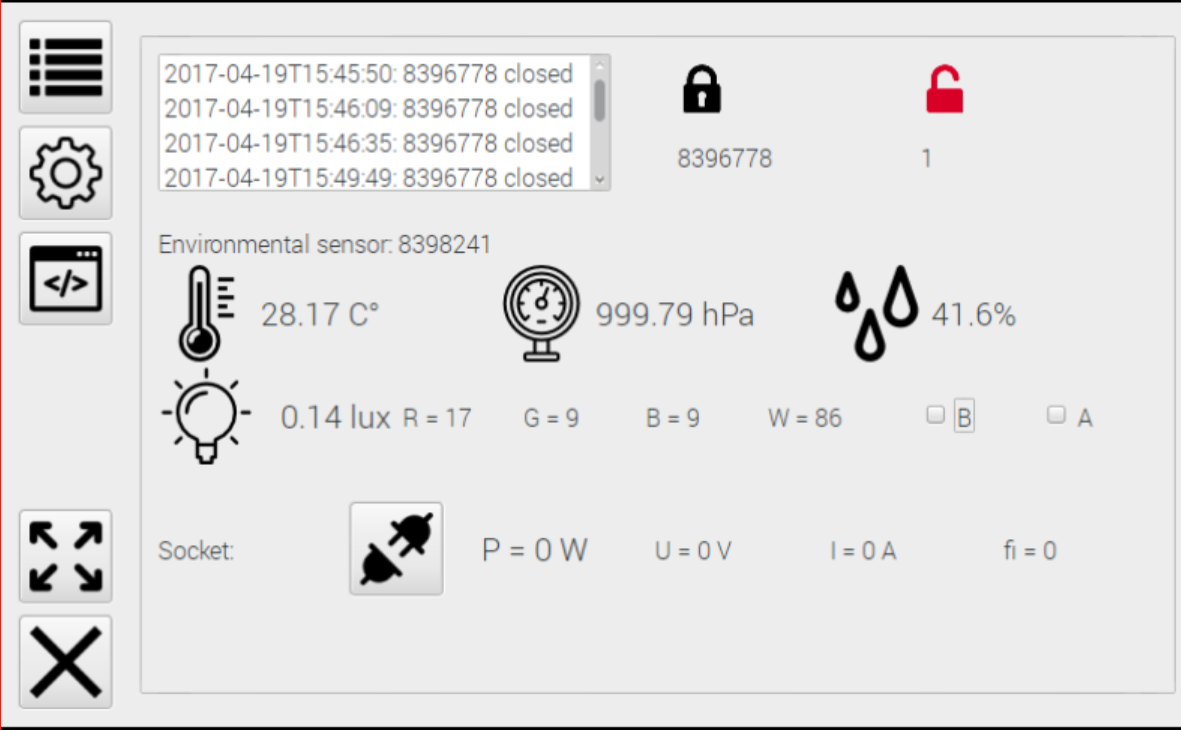
\includegraphics[width=150mm, keepaspectratio]{figures/smarthome-mainpage.png}
	\caption{A k�zponti egys�g f�oldala} 
\end{figure}

\begin{figure}[!ht]
	\centering
	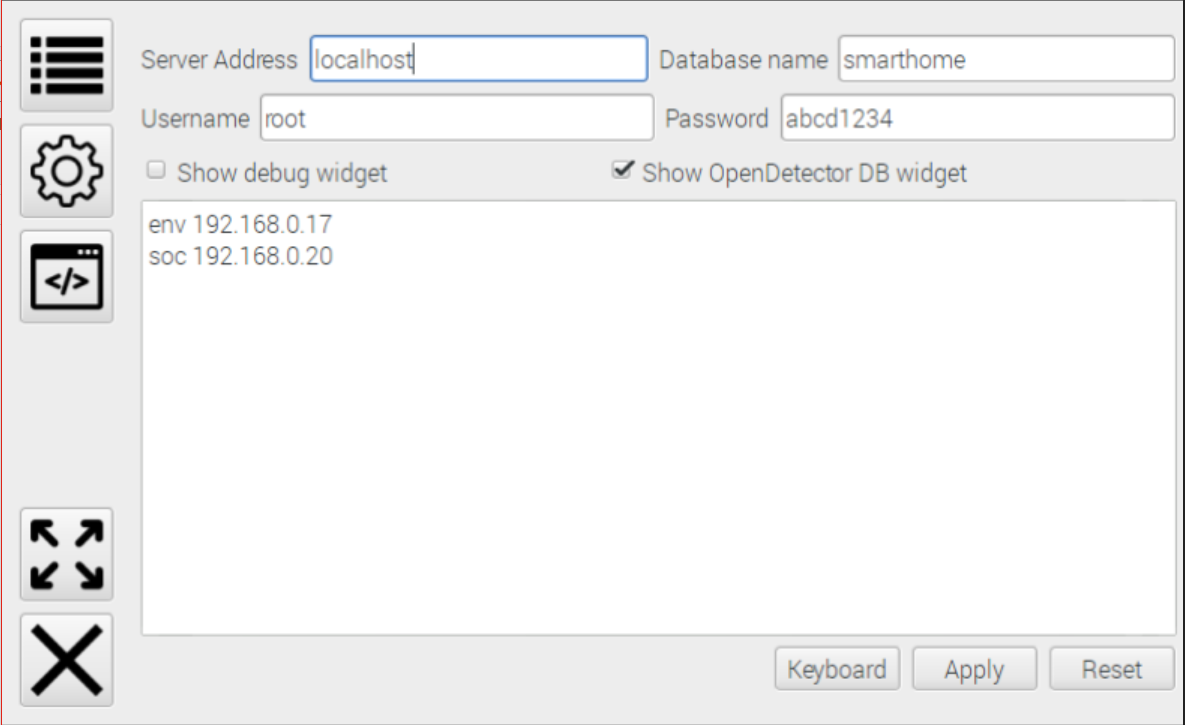
\includegraphics[width=150mm, keepaspectratio]{figures/smarthome-settings.png}
	\caption{A k�zponti egys�g be�ll�t�sai} 
\end{figure}

\begin{figure}[!ht]
	\centering
	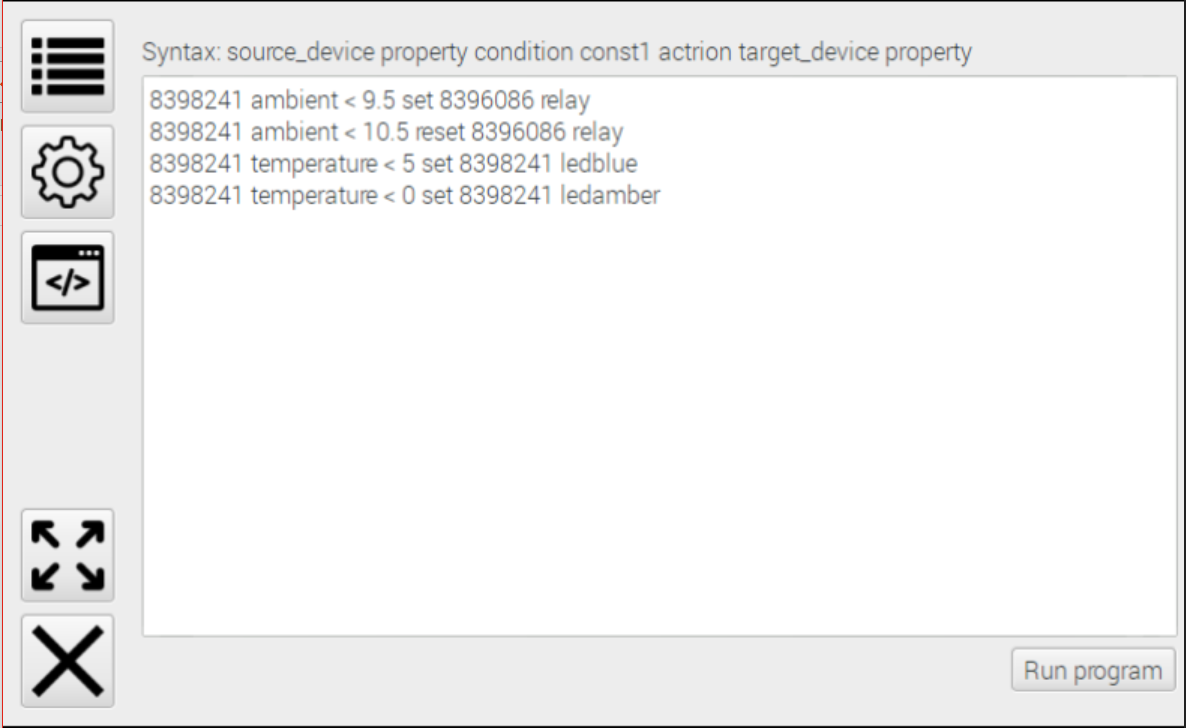
\includegraphics[width=150mm, keepaspectratio]{figures/smarthome-program.png}
	\caption{A k�zponti egys�g programoz� oldala} 
\end{figure}

\begin{figure}[!ht]
\centering
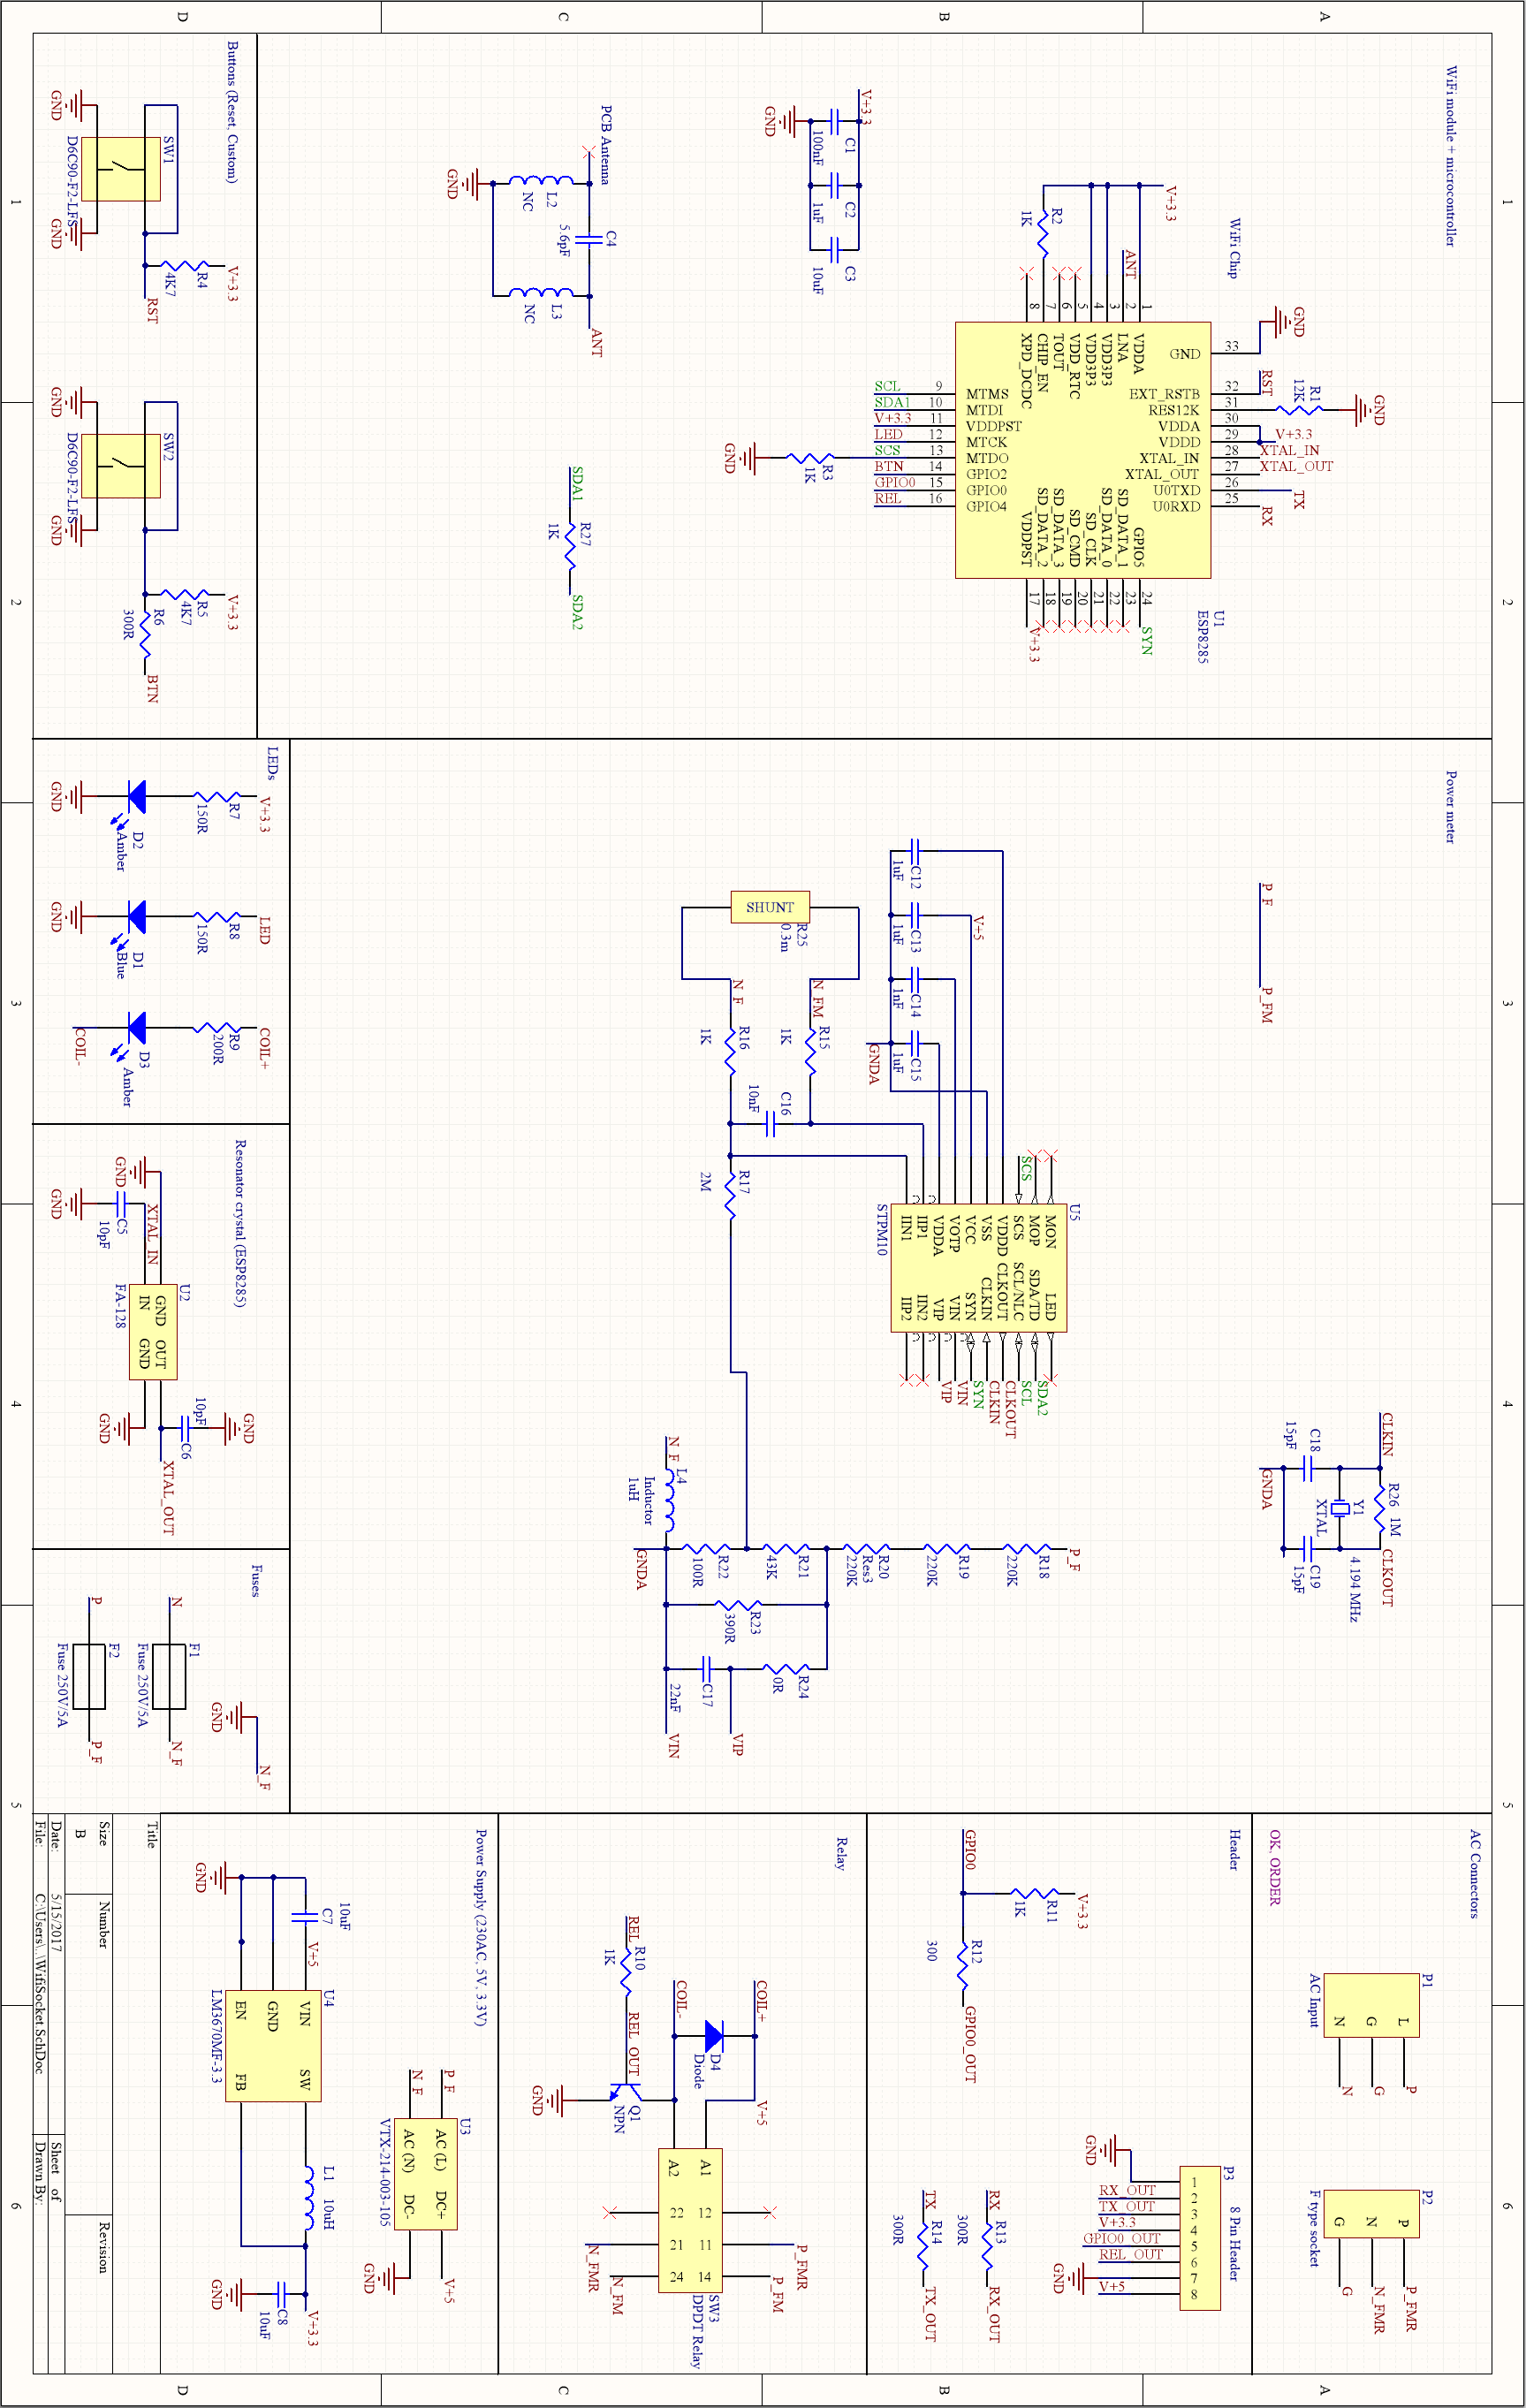
\includegraphics[width=150mm, keepaspectratio]{figures/wifisocket-sch-full.png}
\caption{A programozhat� aljzat kapcsol�si rajza} 
\end{figure}

\begin{figure}[!ht]
	\centering
	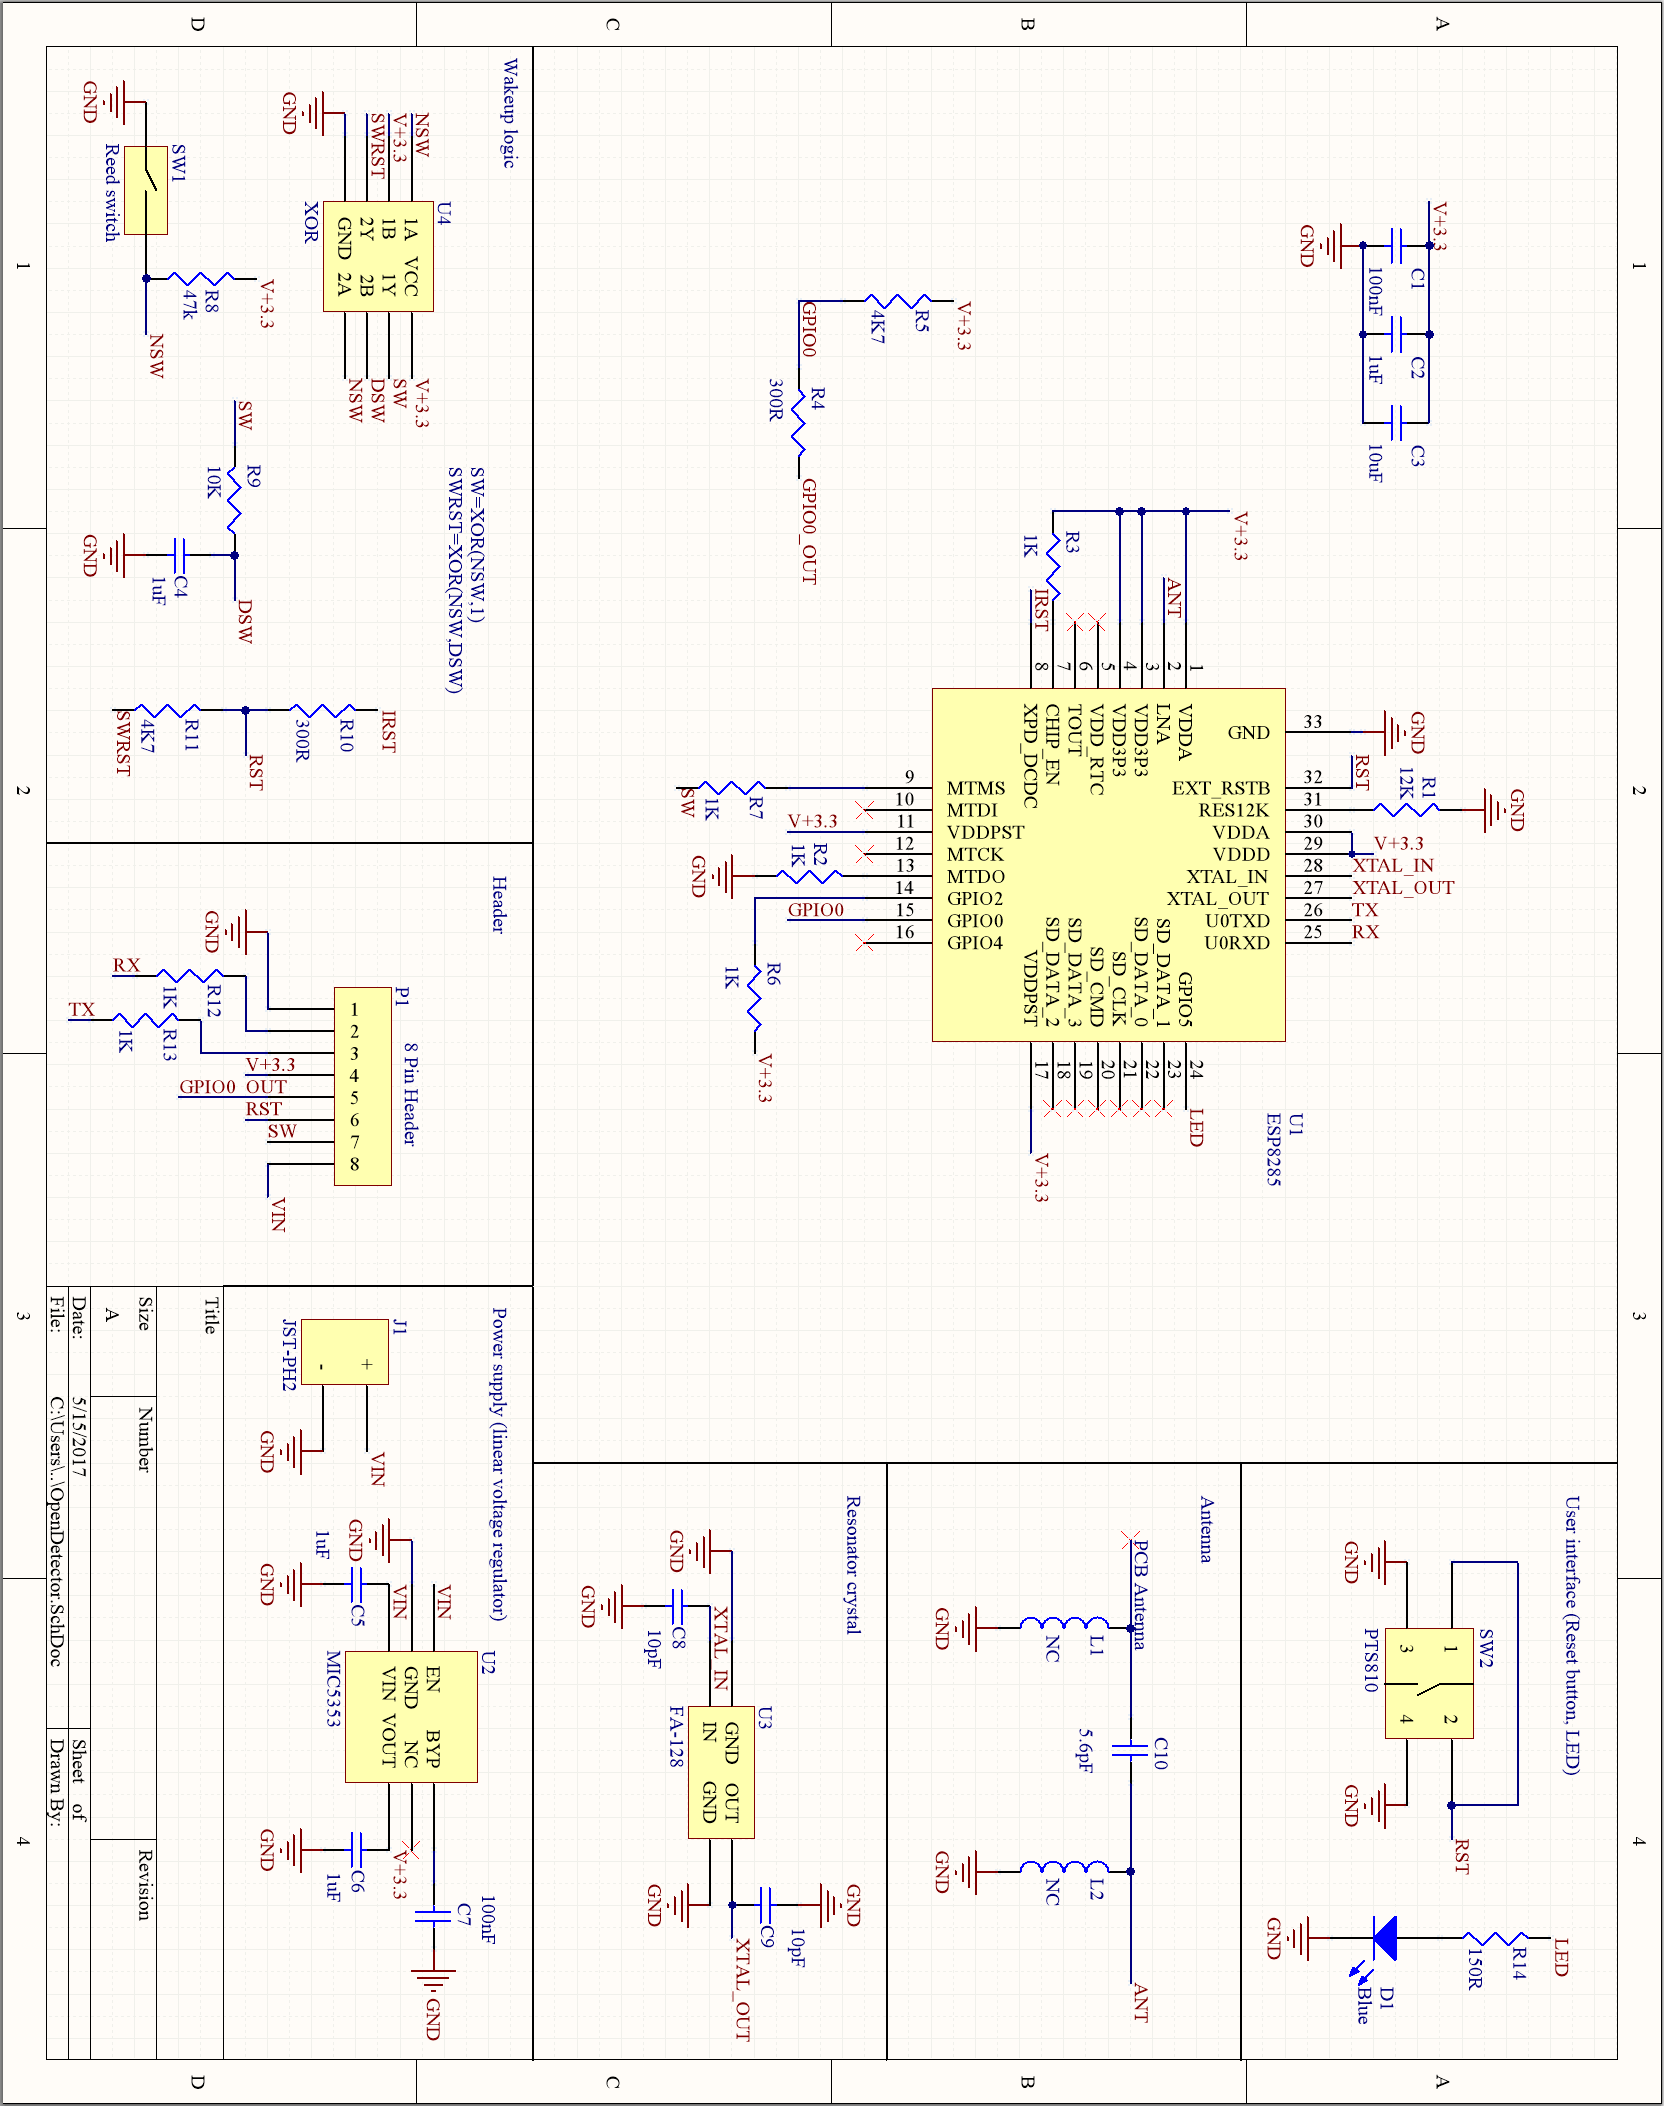
\includegraphics[width=150mm, keepaspectratio]{figures/opendetector-sch-full.png}
	\caption{A nyit�s�rz�kel� kapcsol�si rajza} 
\end{figure}

\begin{figure}[!ht]
	\centering
	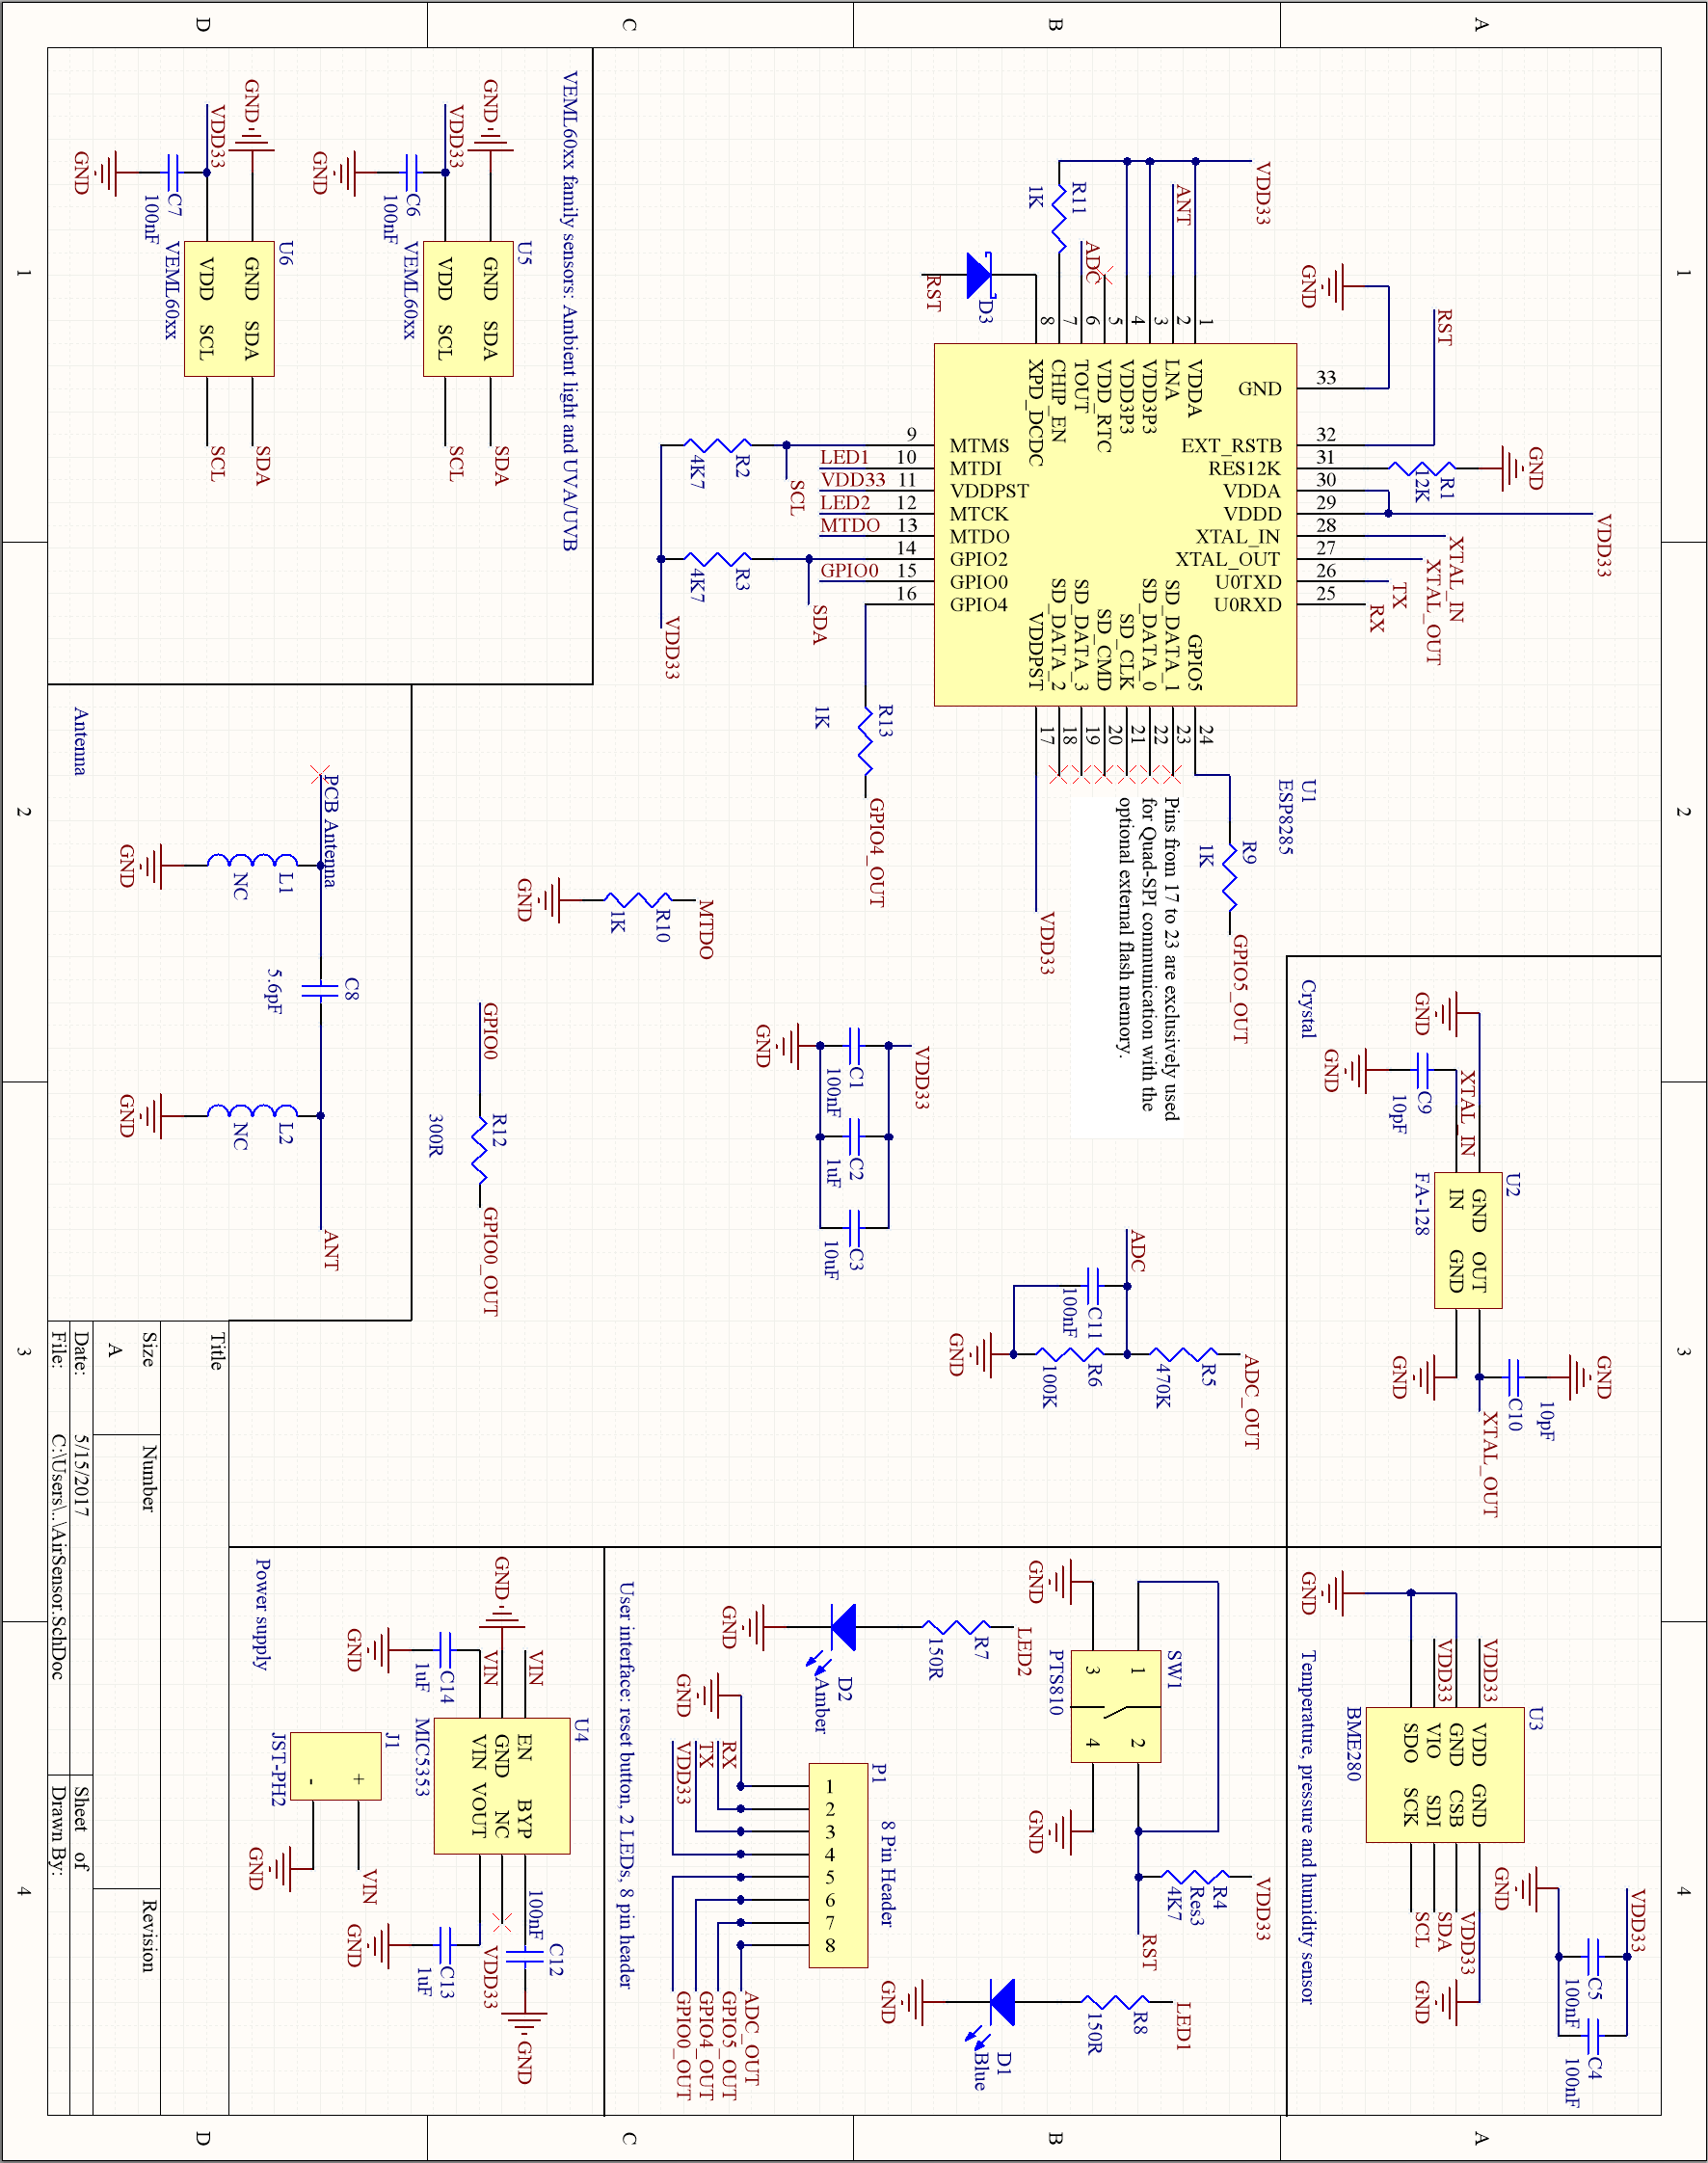
\includegraphics[width=150mm, keepaspectratio]{figures/enviromental-sensor-sch-full.png}
	\caption{A k�rnyezeti szenzor kapcsol�si rajza} 
\end{figure}






